\documentclass[multi=page, tikz, border=2mm]{standalone}
\usepackage{../tikz-preamble}

% arara: pdflatex: { draft: yes }
% arara: pdflatex: { synctex: no }
% arara: latexmk:  { clean: partial }
\begin{document}

\begin{page}
    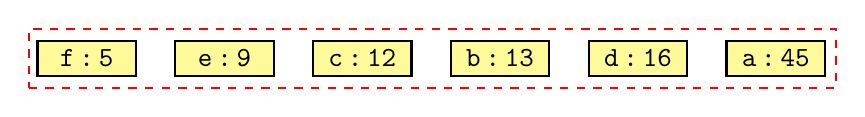
\begin{tikzpicture}[
        level distance=1.25cm,
        level 1/.style={sibling distance=1.75cm},
        level 2/.style={sibling distance=1.75cm},
        level 3/.style={sibling distance=1.75cm},
        thick,
        font=\ttfamily\bfseries
    ]
    \tikzset{
        treenode/.style = {rectangle, draw=black, align=center,fill=yellow!40,minimum width=1.25cm},
    }
    \node[treenode] at (0.00,0) (A) {f\,:\,5};
    \node[treenode] at (1.75,0) (B) {e\,:\,9};
    \node[treenode] at (3.50,0) (C) {c\,:\,12};
    \node[treenode] at (5.25,0) (D) {b\,:\,13};
    \node[treenode] at (7.00,0) (E) {d\,:\,16};
    \node[treenode] at (8.75,0) (F) {a\,:\,45};
    \node[rectangle,anchor=west,minimum width=10.25cm,minimum height=0.75cm,dashed,draw=red] at (-0.75,0) {};
    \end{tikzpicture}
\end{page}

\begin{page}
    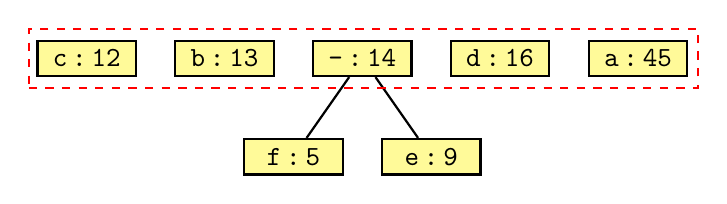
\begin{tikzpicture}[
        level distance=1.25cm,
        level 1/.style={sibling distance=1.75cm},
        level 2/.style={sibling distance=1.75cm},
        level 3/.style={sibling distance=1.75cm},
        thick,
        font=\ttfamily\bfseries
    ]
    \tikzset{
        treenode/.style = {rectangle, draw=black, align=center,fill=yellow!40,minimum width=1.25cm},
    }
    \node[treenode] at (0.00,0) {c\,:\,12};
    \node[treenode] at (1.75,0) {b\,:\,13};
    \node[treenode] at (3.50,0) {-\,:\,14}
        child { node[treenode] {f\,:\,5} }
        child { node[treenode] {e\,:\,9} }
    ;
    \node[treenode] at (5.25,0) {d\,:\,16};
    \node[treenode] at (7.00,0) {a\,:\,45};
    \node[rectangle,anchor=west,minimum width=8.5cm,minimum height=0.75cm,dashed,draw=red] at (-0.75,0) {};
    \end{tikzpicture}
\end{page}

\begin{page}
    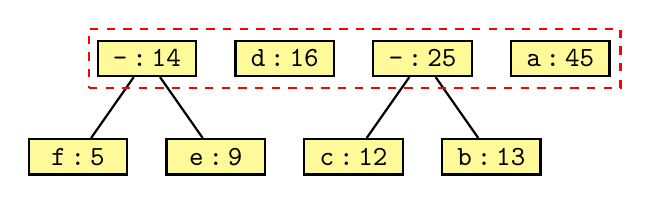
\begin{tikzpicture}[
        level distance=1.25cm,
        level 1/.style={sibling distance=1.75cm},
        level 2/.style={sibling distance=1.75cm},
        level 3/.style={sibling distance=1.75cm},
        thick,
        font=\ttfamily\bfseries
    ]
    \tikzset{
        treenode/.style = {rectangle, draw=black, align=center,fill=yellow!40,minimum width=1.25cm},
    }
    \node[treenode] at (0.0,0) {-\,:\,14}
        child { node[treenode] {f\,:\,5} }
        child { node[treenode] {e\,:\,9} }
    ;
    \node[treenode] at (1.75,0) {d\,:\,16};
    \node[treenode] at (3.50,0) {-\,:\,25}
        child { node[treenode] {c\,:\,12} }
        child { node[treenode] {b\,:\,13} }
    ;
    \node[treenode] at (5.25,0) {a\,:\,45};
    \node[rectangle,anchor=west,minimum width=6.75cm,minimum height=0.75cm,dashed,draw=red] at (-0.75,0) {};
    \end{tikzpicture}
\end{page}

\begin{page}
    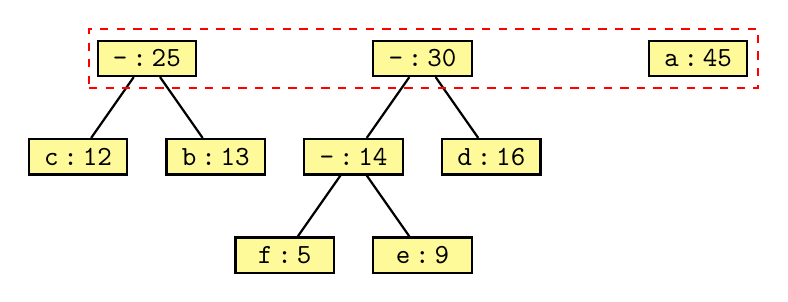
\begin{tikzpicture}[
        level distance=1.25cm,
        level 1/.style={sibling distance=1.75cm},
        level 2/.style={sibling distance=1.75cm},
        level 3/.style={sibling distance=1.75cm},
        thick,
        font=\ttfamily\bfseries
    ]
    \tikzset{
        treenode/.style = {rectangle, draw=black, align=center,fill=yellow!40,minimum width=1.25cm},
    }
    \node[treenode] at (0.0,0) {-\,:\,25}
        child { node[treenode] {c\,:\,12} }
        child { node[treenode] {b\,:\,13} }
    ;
    \node[treenode] at (3.5,0) {-\,:\,30}
        child { node[treenode] {-\,:\,14}
            child { node[treenode] {f\,:\,5} }
            child { node[treenode] {e\,:\,9} }
        }
        child { node[treenode] {d\,:\,16} }
    ;
    \node[treenode] at (7.0,0) {a\,:\,45};
    \node[rectangle,anchor=west,minimum width=8.5cm,minimum height=0.75cm,dashed,draw=red] at (-0.75,0) {};
    \end{tikzpicture}
\end{page}

\begin{page}
    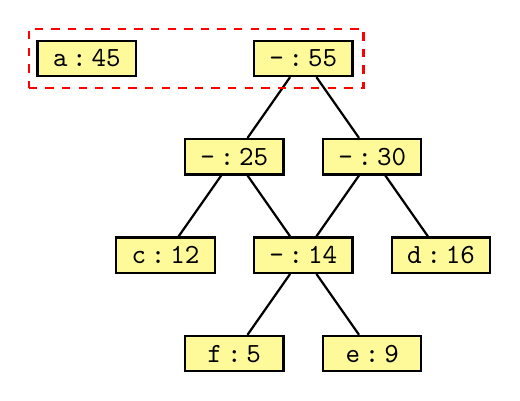
\begin{tikzpicture}[
        level distance=1.25cm,
        level 1/.style={sibling distance=1.75cm},
        level 2/.style={sibling distance=1.75cm},
        level 3/.style={sibling distance=1.75cm},
        thick,
        font=\ttfamily\bfseries
    ]
    \tikzset{
        treenode/.style = {rectangle, draw=black, align=center,fill=yellow!40,minimum width=1.25cm},
    }
    \node[treenode] at (0.0,0) {a\,:\,45};
    \node[treenode] at (2.75,0) {-\,:\,55}
    child { node[treenode]  {-\,:\,25}
        child { node[treenode] {c\,:\,12} }
        child { node[treenode] {b\,:\,13} }
    }
    child { node[treenode]  {-\,:\,30}
        child { node[treenode] {-\,:\,14}
            child { node[treenode] {f\,:\,5} }
            child { node[treenode] {e\,:\,9} }
        }
        child { node[treenode] {d\,:\,16} }
    }
    ;
    \node[rectangle,anchor=west,minimum width=4.25cm,minimum height=0.75cm,dashed,draw=red] at (-0.75,0) {};
    \end{tikzpicture}
\end{page}

\begin{page}
    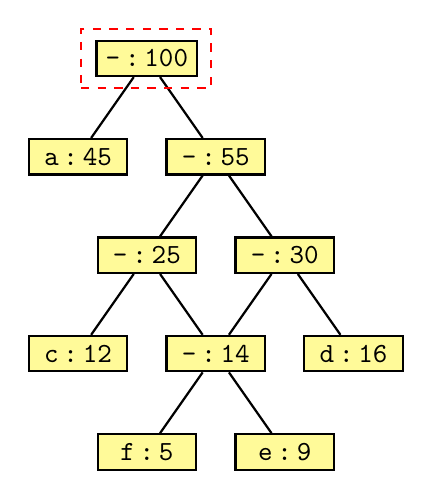
\begin{tikzpicture}[
        level distance=1.25cm,
        level 1/.style={sibling distance=1.75cm},
        level 2/.style={sibling distance=1.75cm},
        level 3/.style={sibling distance=1.75cm},
        thick,
        font=\ttfamily\bfseries
    ]
    \tikzset{
        treenode/.style = {rectangle, draw=black, align=center,fill=yellow!40,minimum width=1.25cm},
    }
    \node[treenode] at (0.0,0) {-\,:\,100}
    child { node[treenode] {a\,:\,45} }
    child { node[treenode] {-\,:\,55}
        child { node[treenode]  {-\,:\,25}
            child { node[treenode] {c\,:\,12} }
            child { node[treenode] {b\,:\,13} }
        }
        child { node[treenode]  {-\,:\,30}
            child { node[treenode] {-\,:\,14}
                child { node[treenode] {f\,:\,5} }
                child { node[treenode] {e\,:\,9} }
            }
            child { node[treenode] {d\,:\,16} }
        }
    }
    ;
    \node[rectangle,anchor=west,minimum width=1.65cm,minimum height=0.75cm,dashed,draw=red] at (-0.85,0) {};
    \end{tikzpicture}
\end{page}

\begin{page}
    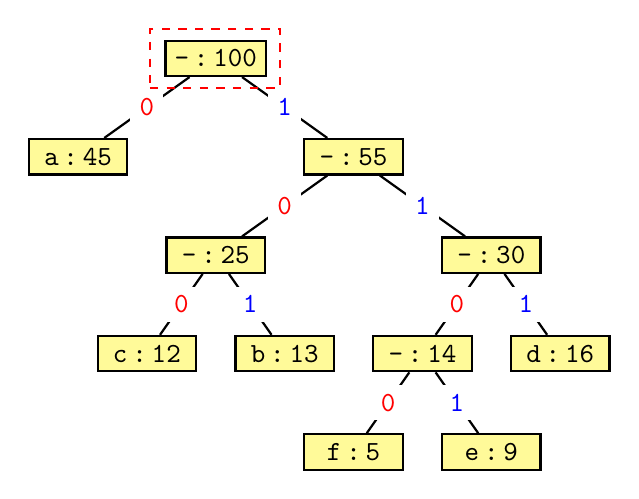
\begin{tikzpicture}[
        level distance=1.25cm,
        level 1/.style={sibling distance=3.5cm},
        level 2/.style={sibling distance=3.50cm},
        level 3/.style={sibling distance=1.75cm},
        level 4/.style={sibling distance=1.75cm},
        thick,
        font=\ttfamily\bfseries
    ]
    \tikzset{
        treenode/.style = {rectangle, draw=black, align=center,fill=yellow!40,minimum width=1.25cm},
        edgestyleL/.style = {midway, fill=white,draw=none,font={\ttfamily},text=red},
        edgestyleR/.style = {midway, fill=white,draw=none,font={\ttfamily},text=blue}
    }
    \node[treenode] at (0.0,0) {-\,:\,100}
    child { node[treenode] {a\,:\,45} edge from parent node[edgestyleL] {0} }
    child { node[treenode] {-\,:\,55}
        child { node[treenode]  {-\,:\,25}
        child { node[treenode] {c\,:\,12} edge from parent node[edgestyleL] {0} }
        child { node[treenode] {b\,:\,13} edge from parent node[edgestyleR] {1}}
        edge from parent node[edgestyleL] {0} }
        child { node[treenode]  {-\,:\,30}
            child { node[treenode] {-\,:\,14}
                child { node[treenode] {f\,:\,5} edge from parent node[edgestyleL] {0} }
                child { node[treenode] {e\,:\,9} edge from parent node[edgestyleR] {1} }
                edge from parent node[edgestyleL] {0}
            }
            child { node[treenode] {d\,:\,16} edge from parent node[edgestyleR] {1}}
            edge from parent node[edgestyleR] {1}
        }
        edge from parent node[edgestyleR] {1}
    }
    ;
    \node[rectangle,anchor=west,minimum width=1.65cm,minimum height=0.75cm,dashed,draw=red] at (-0.85,0) {};
    \end{tikzpicture}
\end{page}

\end{document}